\documentclass{beamer}
%\usepackage[latin1]{inputenc}
\usetheme{Warsaw}
\title[Intro to Python: Week 9]{Introduction  to Python\\ 
Decorators, Context Managers, \\
Packages and Packaging}
\author{Christopher Barker}
\institute{UW Continuing Education}
\date{December 3, 2013}

\usepackage{listings}
\usepackage{hyperref}

\begin{document}

% ---------------------------------------------
\begin{frame}
  \titlepage
\end{frame}

% ---------------------------------------------
\begin{frame}
\frametitle{Table of Contents}
%\tableofcontents[currentsection]
  \tableofcontents
\end{frame}


\section{Review/Questions}

% ---------------------------------------------
\begin{frame}{Review of Previous Class}

\begin{itemize}
  \item Magic methods
  \item Iterators
  \item Generators
  \item (wxPython)
\end{itemize}

\end{frame}


% ---------------------------------------------
\begin{frame}{Lightning Talks}

\vfill
{\LARGE Lightning talks today:}

\vfill
{\Large

\vfill
 Harlan AuBuchon
\vfill
  Luke Cypret
\vfill
 Brian Schmitz
\vfill

}
\vfill

\end{frame}


% ---------------------------------------------
\begin{frame}{Review}

  \vfill
  {\Large Questions about labs? }

  \vfill
  {\Large My Solutions? }

  \vfill

\end{frame}

\begin{frame}[fragile]{A diversion...}

\Large{A number of you are already using \verb|iPython|}

\vfill
\Large{It's a very useful tool}

\vfill
\Large{And the \verb|iPython| notebook is even cooler .. paticularly for in-class demos.}

\vfill
\Large{So I'll use it some today:}

\vfill
\url{http://ipython.org/ipython-doc/dev/interactive/notebook.html}


\end{frame}


%########################
\section{Decorators}

% ---------------------------------------------
\begin{frame}[fragile]{Decorators}

{\LARGE Decorators are wrappers around functions}

\vfill
{\LARGE They let you add code before and after the execution of a function}

\vfill
{\LARGE Creating a custom version of that function}

\end{frame} 

% ---------------------------------------------
\begin{frame}[fragile]{Decorators}

{\LARGE Syntax:}

\vfill
\begin{verbatim}
@logged
def add(a, b):
    """add() adds things"""
    return a + b
\end{verbatim}

\vfill
{\Large Demo and Motivation: \\
\verb|code/decorators/basic_math.py [ipnb]| }

\vfill
PEP: \url{http://www.python.org/dev/peps/pep-0318/}

\end{frame} 

% ---------------------------------------------
\begin{frame}[fragile]{Decorators}

{\LARGE \verb|@| decorator operator is an abbreviation:}

{\large
\vfill
\begin{verbatim}
@f
def g:
    pass
\end{verbatim}

\vfill
same as

\vfill
\begin{verbatim}
def g:
    pass
g = f(g)
\end{verbatim}
}

\vfill
{\Large ``Syntactic Sugar'' -- but really quite nice}

\end{frame} 

% ---------------------------------------------
\begin{frame}[fragile]{Decorators}

{\LARGE demo:

\vfill
\begin{verbatim}
decorator.py
\end{verbatim}

}
\end{frame} 

% ---------------------------------------------
\begin{frame}[fragile]{Decorator  examples}

{\LARGE Examples from the stdlib:}

\vfill
{\Large Does this structure:}

\vfill
\begin{verbatim}
def g:
    pass
g = f(g)
\end{verbatim}

\vfill

{\Large look familiar from last class?}
\end{frame} 

% ---------------------------------------------
\begin{frame}[fragile]{Decorator examples}

{\LARGE \verb|staticmethod()|}

\vfill
\begin{verbatim}
class C(object):
    def add(a, b):
        return a + b
    add = staticmethod(add)
\end{verbatim}

\vfill

\end{frame} 

% ---------------------------------------------
\begin{frame}[fragile]{Decorator examples}

{\LARGE \verb|staticmethod()|}

\vfill
{\Large Decorator form:}
\begin{verbatim}
class C(object):
    @staticmethod
    def add(a, b):
        return a + b
\end{verbatim}

\vfill

{\LARGE ( and \verb|classmethod| )}
\end{frame} 

% ---------------------------------------------
\begin{frame}[fragile]{examples}

{\LARGE \verb|property()|}

\vfill
\begin{verbatim}
class C(object):
    def __init__(self):
        self._x = None
    def getx(self):
        return self._x
    def setx(self, value):
        self._x = value
    def delx(self):
        del self._x
    x = property(getx, setx, delx,
                 "I'm the 'x' property.")
\end{verbatim}

\vfill
{\large becomes...}
\end{frame} 

% ---------------------------------------------
\begin{frame}[fragile]{Decorator examples}

\begin{verbatim}
class C(object):
    def __init__(self):
        self._x = None
    @property
    def x(self):
        return self._x
    @x.setter
    def x(self, value):
        self._x = value
    @x.deleter
    def x(self):
        del self._x
\end{verbatim}

\vfill
{\large Puts the info close to where it is used}
\end{frame} 

% ---------------------------------------------
\begin{frame}[fragile]{examples}

{\LARGE CherryPy}

\vfill
\begin{verbatim}
import cherrypy
class HelloWorld(object):
    @cherrypy.expose
    def index(self):
        return "Hello World!"
cherrypy.quickstart(HelloWorld())
\end{verbatim}

\end{frame} 

% ---------------------------------------------
\begin{frame}[fragile]{examples}

{\LARGE Pyramid}

\vfill
\begin{verbatim}

@template
def A_view_function(request)
   .....
@json
def A_view_function(request)
   ......


\end{verbatim}

so you don't need to think about what your view is returning...

\end{frame} 


% ---------------------------------------------
\begin{frame}[fragile]{decorators...}

{\Large For this class:}

\vfill
{\Large Mostly want to you to know how to use decorators that someone else has written}

\vfill
{\Large Have a basic idea what they do when you do use them}

\vfill
{\Large But writing a couple will help you ``get'' it, and help cement your Python knowledge...}


\end{frame} 

% ---------------------------------------------
\begin{frame}[fragile]{Writing Decorators}

{\LARGE So how to you write one?}

\vfill
{\Large
demo in iPython notebook

\vfill
\begin{verbatim}
code\decorators\DecoratorDemo.py
\end{verbatim}
}

\vfill
{\large For more detail: (and talks about closures...):}\\

\url{http://simeonfranklin.com/blog/2012/jul/1/python-decorators-in-12-steps/}

\end{frame} 


%-------------------------------
\begin{frame}[fragile]{LAB}

\begin{itemize}
  \item Re-write the properties from last week's \verb|Circle| class
        to use the decorator syntax (see a couple slides back for an example)\\
        (\verb|circle_properties.py| and \verb|test_circle_properties.py|)
  \item Write a decorator that can be used to wrap any function that returns a string in a \verb|<p>| element -- auto-generation of simple html.
 (\verb|p_wrapper.py|)      

  \item Try using a class to make a decorator that will wrap a
   specified tag around a function that returns a string:
   \begin{verbatim}
   @tag_wrapper('h1')
   def func2(x, y=4, z=2):
       return "the sum of %s and %s and %s is %s"%(x, y, z, x+y+z)
   >>> print func2(3,4)
   <h1> the sum of 3 and 4 and 2 is 9 </h1>
   \end{verbatim}
\end{itemize}

\end{frame}

%-------------------------------
\begin{frame}{Lightning Talks}

{\LARGE Lightning Talks:}

\vfill
{\Large  Harlan AuBuchon}

\vfill
{\Large  Luke Cypret}

\end{frame}

%%%%%%%%%%%%%%%%%%%%%%%%%%%%%%
\section{Context Managers}

%----------------------------------------
\begin{frame}[fragile]{Context Managers}

{\LARGE the \verb|with| statement}

\vfill
{\Large A class with \verb|__enter__()| and \verb|__exit__()| methods.}
 
\vfill
{\Large \verb|__enter__()| is run before your block of code}

\vfill
{\Large \verb|__exit__()| is run after your block of code}

\vfill
{\Large Can be used to setup/cleanup before and after: open/closing files, db connections, etc}
\end{frame} 

%----------------------------------------
\begin{frame}[fragile]{Context Managers}

{\Large ``PEP 343: the \verb|with| statement''} \\
\hspace{0.2in}  -- A.M. Kuchling

\url{http://docs.python.org/dev/whatsnew/2.6.html#pep-343-the-with-statement}

\vfill
{\Large ``Understanding Python's \verb|with| statement''} \\
\hspace{0.2in}  -- Fredrik Lundh 

\url{http://effbot.org/zone/python-with-statement.htm}

\vfill
{\Large ``The Python \verb|with| Statement by Example''} \\
\hspace{0.2in}  -- Jeff Preshing 

\url{http://preshing.com/20110920/the-python-with-statement-by-example}

\end{frame} 


%----------------------------------------
\begin{frame}[fragile]{Context Managers}

{\Large Use syntax:}

\begin{verbatim}
with manager as something:
    a = block_of_code
    use_something_here(something)
    ...
\end{verbatim}

\vfill
{\large
\verb`manager` is the context manager: i.e. has an \verb`__enter__` and \verb`__exit__` method -- if \verb`__enter__` returns an object, it gets assigned to \verb`something`
}

\vfill
\end{frame} 

%----------------------------------------
\begin{frame}[fragile]{Context Managers}

{\Large The file object is also a context manager:}

\begin{verbatim}
with open(filename) as the_file:
    for line in the_file:
        work_with(line)
        ...
     ...
\end{verbatim}

\vfill

{\Large In this case, the file will automatically be closed when you leave that block, regardless of errors, etc.}
\vfill

{\Large Most commonly used context manager -- by far!}

\end{frame} 

%----------------------------------------
\begin{frame}[fragile]{Context Managers}

{\Large You also may hav seen this in some of my unit tests:}

\begin{verbatim}
with pytest.raises(ZeroDivisionError):
    some_test_code_here
    1/0
\end{verbatim}

\vfill

{\Large Context Managers can also catch Exceptions....}
\vfill

\end{frame} 

%-------------------------------
\begin{frame}[fragile]{LAB}

{\Large See if you can write a context manger that will time some code.}

{\large When using it, you can do:}
\begin{verbatim}
  with timer:
      this_is_some_code_to_run()
      how_long_might_it_take
\end{verbatim}

{\large and you'll get something like:}

\begin{verbatim}
  this code took 0.12 seconds
\end{verbatim}

\vfill
{\large See: \verb`context_manager\timer_context.html` (\verb`timer_context.py`) }

\end{frame}

%-------------------------------
\begin{frame}{Lightning Talk}

{\LARGE Lightning Talk:}

\vfill
{\large   Brian Schmitz}

\end{frame}


\section{Packages and Packaging}

% ---------------------------------------------
\begin{frame}[fragile]{Modules and Packages}

\vfill
{\Large A module is a file with python code in it}

\vfill
{\Large A package is a directory with an \verb|__init__.py| file in it}

\vfill
{\Large And usually other modules, packages, etc...}

\begin{verbatim}
my_package
    __init__.py
    module_a.py
    module_b.py
\end{verbatim}

\begin{verbatim}
import my_package
\end{verbatim}

runs \verb|my_package/__init__.py|

\end{frame} 


% ---------------------------------------------
\begin{frame}[fragile]{Modules and Packages}

\vfill
\begin{verbatim}
import sys

for p in sys.path:
    print p

\end{verbatim}

\vfill
(demo)
\end{frame} 

% ---------------------------------------------
\begin{frame}[fragile]{Installing Python}

{\Large Linux:}

Usually part of the system -- just use it

\vfill
{\Large Windows:}

\vfill
Use the \url{python.org} version:

\vfill
System Wide

\vfill
Can install multiple versions if need be

\vfill
Third party binaries for it.

\end{frame} 

% ---------------------------------------------
\begin{frame}[fragile]{Installing Python}

{\Large OS-X:}

Comes with the system, but:
\begin{itemize}
    \item Apple has never upgraded within a release
    \item There are non-open source components
    \item Third party packages may or may not support it
    \item Apple does use it -- so don't mess with it.
    \item I usually recommend the \url{python.org} version
\end{itemize}
(Also Macports, Fink, Home Brew...)

\vfill
\end{frame} 

% ---------------------------------------------
\begin{frame}[fragile]{Distributions}

\vfill
{\Large There are also a few ``curated'' distributions:}

\vfill
{\Large These provide python and a package management system for hard-to-buid packages.}

\vfill
{\Large Widely used by the scipy community (lots of hard to build stuff that needs to work together...)}

{\large
\begin{itemize}
  \item Anoconda (\url{https://store.continuum.io/cshop/anaconda/})
  \item Canopy (\url{https://www.enthought.com/products/canopy/})
  \item ActivePython (\url{http://www.activestate.com/activepython})
\end{itemize}
}

\end{frame} 

% ---------------------------------------------
\begin{frame}[fragile]{Installing Packages}

{\Large Every Python installation has its own stdlib and \verb|site-packages| folder}

\vfill
{\Large\verb|site-packages| is the default place for third-party packages}

\end{frame} 

% ---------------------------------------------
\begin{frame}[fragile]{Finding Packages}

{\Large The Python Package Index:}

\vfill
{\LARGE PyPi}

\vfill
\url{http://pypi.python.org/pypi}

\end{frame} 

% ---------------------------------------------
\begin{frame}[fragile]{Installing Packages}

{\Large From source}
(\verb|setup.py install|)

\vfill
{\Large With the system installer (apt-get, yum, etc...)}

\vfill
{\Large From binaries: }

\vfill
{\Large Windows:} MSI installers

\vfill
{\Large OS-X:} dmg installers 

\vfill
{\Large And now:} binary wheels

(make sure to get compatible packages)

\vfill
{\Large \verb|easy_install| and \verb|pip|}

\end{frame} 

% ---------------------------------------------
\begin{frame}[fragile]{Installing Packages}

{\Large In the beginning, there was the \verb|distutils|:}

\url{....}

{\Large But \verb|distutils| is missing some key features:}
\begin{itemize}
  \item package versioning
  \item package discovery
  \item auto-install
\end{itemize}

\vfill
{\Large - And then came \verb|PyPi|}

\vfill
{\Large - And then came \verb|setuptools|}

\vfill
{\Large - But that wasn't well maintained...}

\vfill
{\Large - Then there was \verb|distribute/pip|}

\vfill
{\Large - Which has now been merged back into \verb|setuptools|}

\end{frame} 

% ---------------------------------------------
\begin{frame}[fragile]{Installing Packages}

\vfill
{\LARGE Actually, it's still a bit of a mess}
\vfill
{\large But getting better...}
\end{frame} 

% ---------------------------------------------
\begin{frame}[fragile]{Packaging Time line}

{\centering
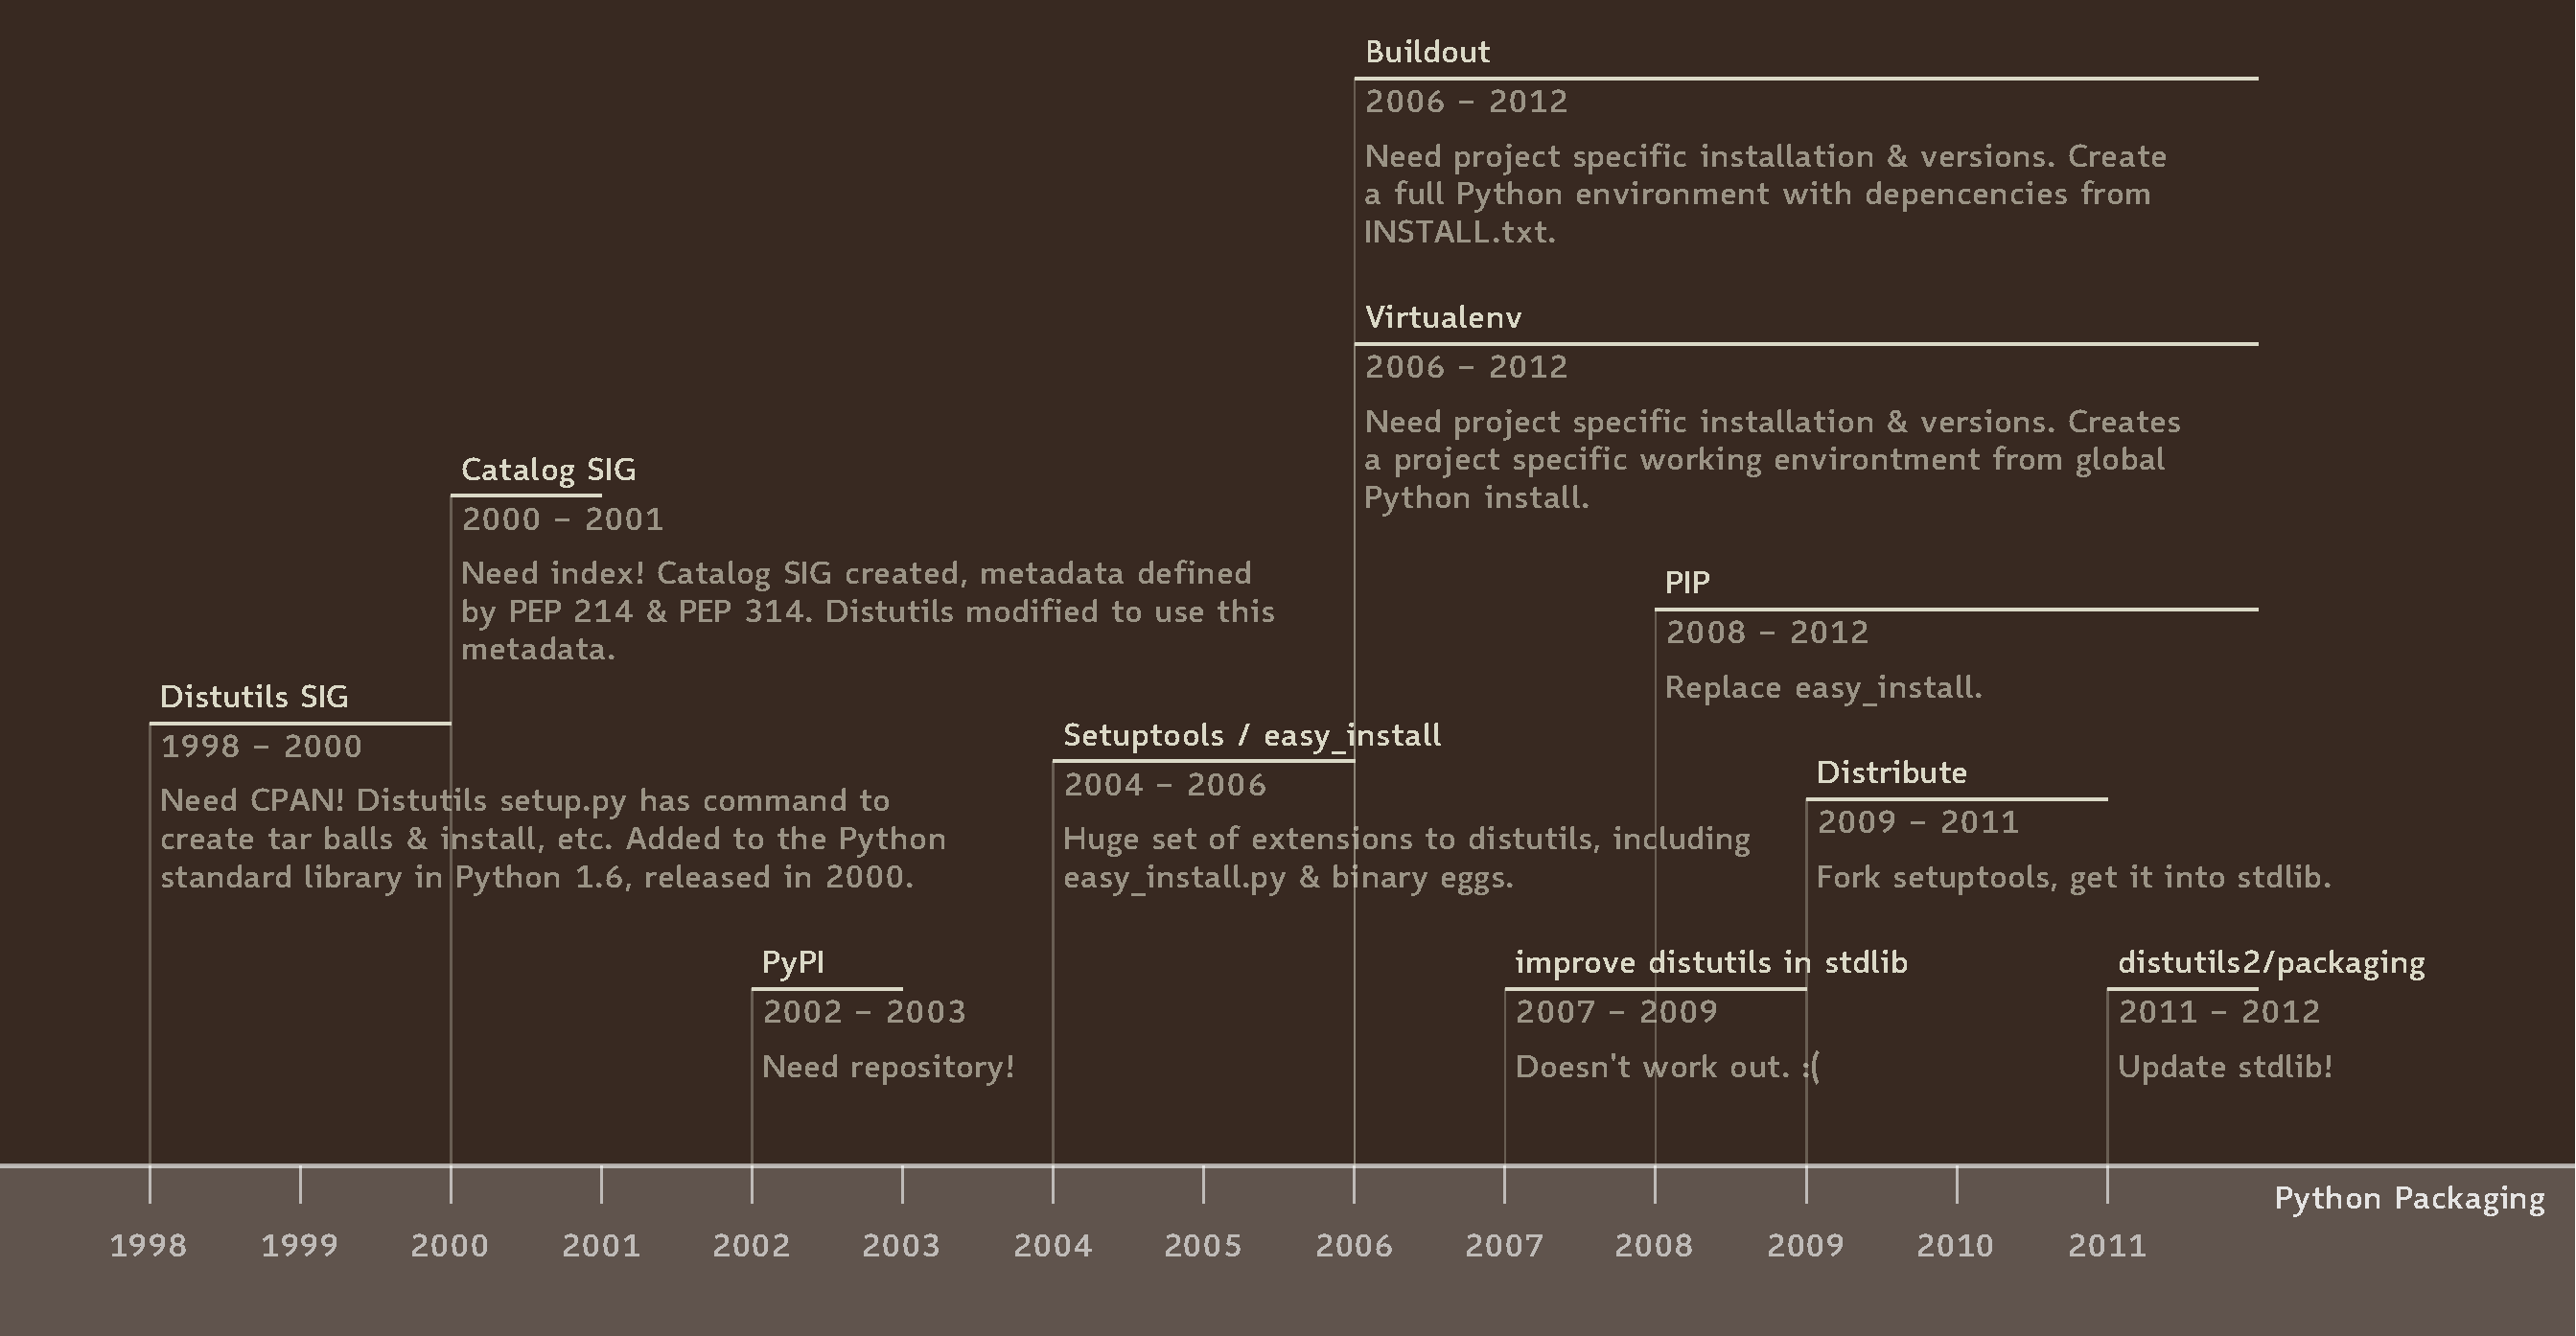
\includegraphics[width=4.5in]{PackagingTimeline.pdf}
}
\end{frame} 

% ---------------------------------------------
\begin{frame}[fragile]{Packaging Tools}

{\centering
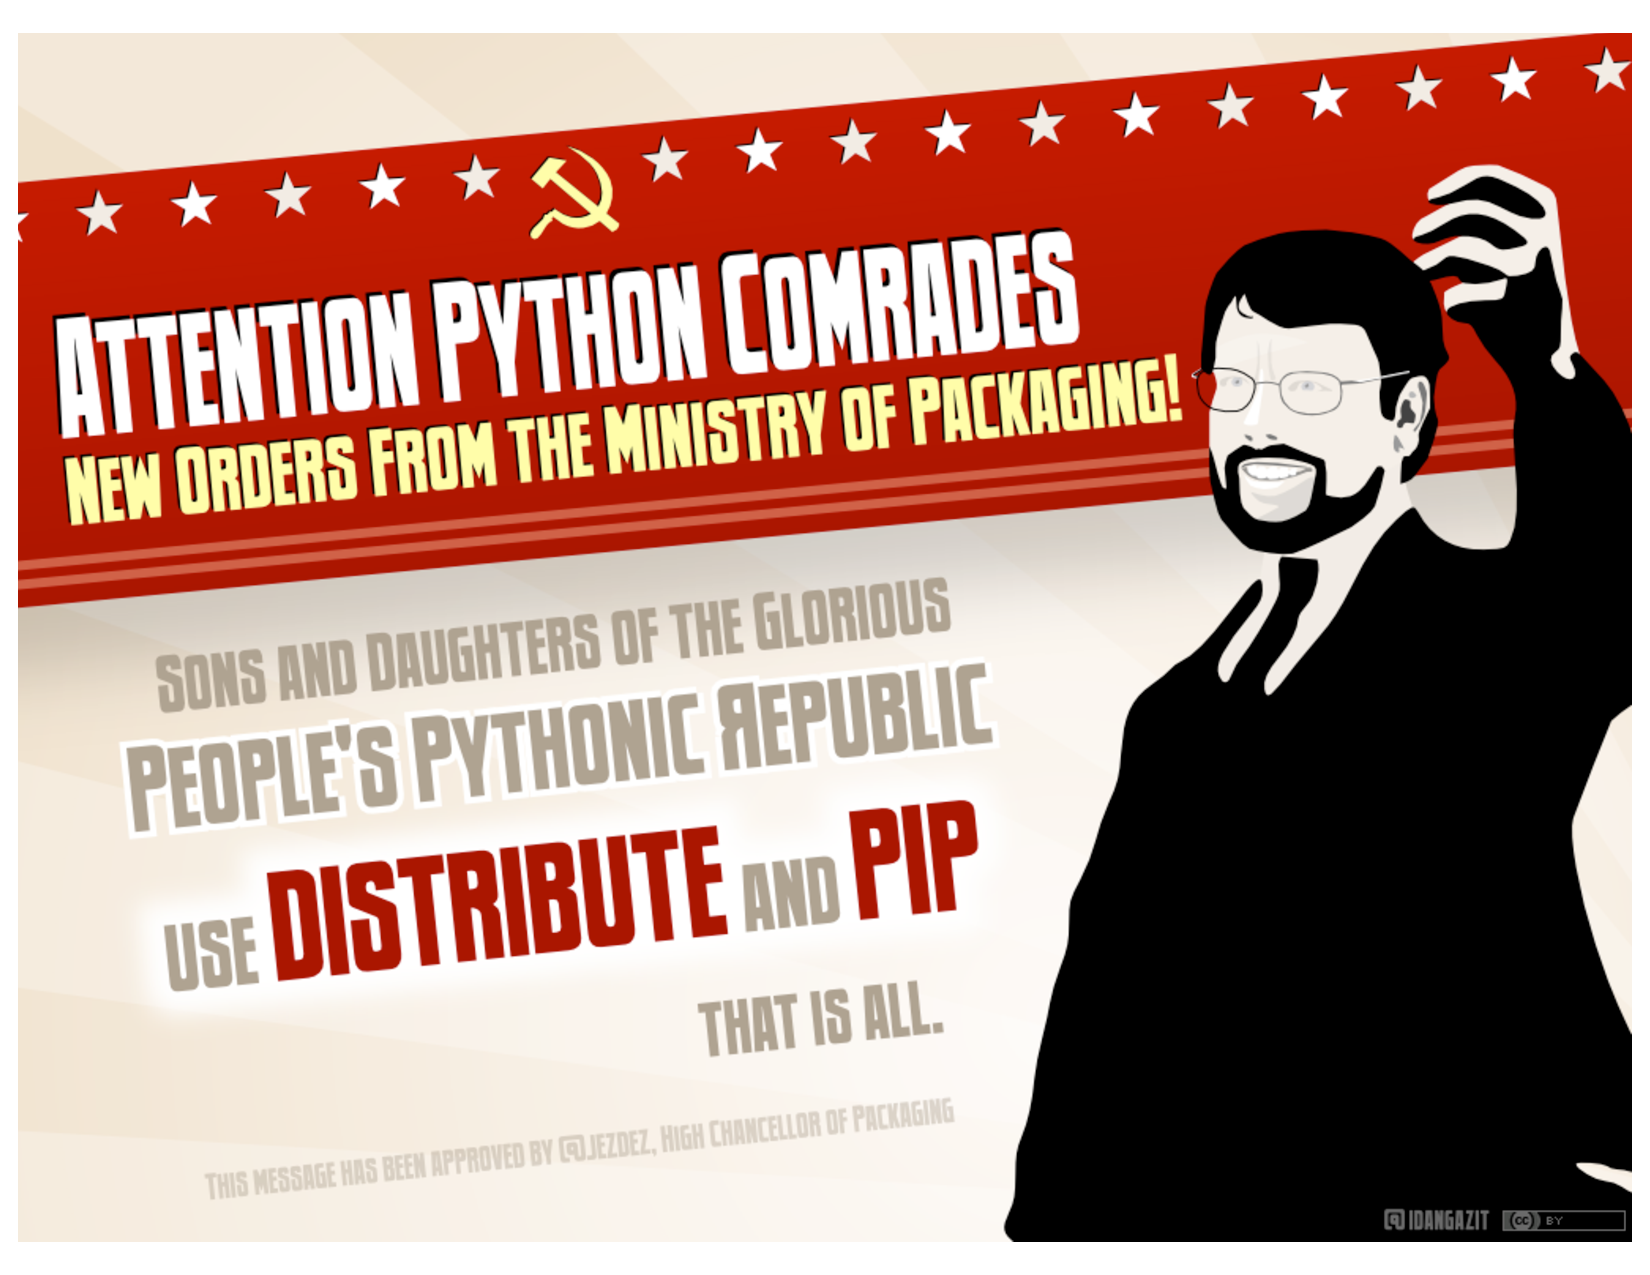
\includegraphics[width=4.5in]{packaging1.pdf}
}

\end{frame} 

% ---------------------------------------------
\begin{frame}[fragile]{Current State of Packaging}

\vfill
{\Large To build packages: distutils}

\url{http://docs.python.org/2/distutils/}

\vfill
{\Large For more features: setuptools}

\url{http://pythonhosted.org/setuptools/}

\vfill
{\Large To install packages: pip}

\url{http://www.pip-installer.org/en/latest/}

\vfill
{\Large For binary packages: wheels}

\url{http://www.python.org/dev/peps/pep-0427/}


\end{frame} 

% ---------------------------------------------
\begin{frame}[fragile]{Compiled Packages}

{\LARGE Biggest issue is with compiled extensions\\[0.1in]
\hfill(C/C++, etc)\hfill
}
\vfill
{\Large -- You need the right compiler set up}

\vfill
{\LARGE Dependencies}

\vfill
{\Large -- Here's were it gets really ugly}

\vfill
{\Large -- Particularly on Windows}

\end{frame} 

% ---------------------------------------------
\begin{frame}[fragile]{Compiled Packages}

{\LARGE Linux}

\vfill
{\Large Pretty straightforward:}

\vfill
{\Large 1) Is there a system package \\[0.1in] (rpm, deb, apt-get, etc...)?
}

\vfill
{\Large 2) Install the dependencies, build from source:\\[0.1in]
\verb`python setup.py build ; python setup.py install` 

\vfill
( Or maybe \verb`pip install` will just work )
}

\end{frame} 

% ---------------------------------------------
\begin{frame}[fragile]{Compiled Packages}

{\LARGE Windows}

\vfill
{\Large Sometimes simpler:}

\vfill
{\Large 1) A lot of packages have Windows binaries:\\[0.1in]
            - Usually for \url{python.org} builds \\[0.1in]
            - Excellent source:} \url{http://www.lfd.uci.edu/~gohlke/pythonlibs/} \\[0.1in]
{\Large            - Make sure you get 32 or 64 bit consistent
}

\vfill
{\Large 2) But if no binaries: \\[0.1in]
           - Hope the dependencies are available!\\[0.1in]
           - Set up the compiler (MS VS2008 Express works)
}

\end{frame} 

% ---------------------------------------------
\begin{frame}[fragile]{Compiled Packages}

{\LARGE OS-X}

\vfill
{\Large Lots of Python versions:\\[0.1in]
  - Apple's built-in (different for each version of OS)\\[0.1in]
  - \url{python.org} builds.\\
  \hspace{0.5in}- 32 bit PPC+Intel\\
  \hspace{0.5in}- 32+64 bit Intel\\[0.1in]
  - Macports
  - Homebrew
}


\vfill
{\Large Binary Installers (dmg or wheel) have to match python version}

\end{frame} 

% ---------------------------------------------
\begin{frame}[fragile]{Compiled Packages}

{\LARGE OS-X}

\vfill
{\Large If you have to build it yourself:}

\vfill
{\Large Xcode compiler (the right version):\\[0.1in]
  - Version 3.* for 32 bit PPC+Intel\\[0.1in]
  - Version 4.* for 32+64 bit Intel\\
}

\vfill
{\Large If extra dependencies:\\[0.1in]
  - macports or home brew often easiest way to build them
}

\end{frame} 

% ---------------------------------------------
\begin{frame}[fragile]{Final Recommendation}

{\Large First try: \verb|pip install|}

\vfill
{\Large If that doesn't work:}

\vfill
{\Large Read the docs of the package you want to install}

\vfill
{\Large Do what they say}

\end{frame} 

% ---------------------------------------------
\begin{frame}[fragile]{virtualenv}

{\Large \verb|virtualenv| is a tool to create isolated Python environments.}

\vfill
{\Large Very useful for developing multiple apps}

\vfill
{\Large Or deploying more than one on one system}

\vfill
\url{http://www.virtualenv.org/en/latest/index.html}

\vfill
(Cris will get into more detail with this next class)

\end{frame} 


\section{Distributing}

\begin{frame}[fragile]{Distributing}

{\LARGE What if you need to distribute you own:}

\vfill
{\Large Scripts}

\vfill
{\Large Libraries }

\vfill
{\Large Applications }
\vfill

\end{frame} 

\begin{frame}[fragile]{Scripts}

\vfill
{\LARGE Often you can just copy, share, or check in the script to source
control and call it good.}

\vfill
{\Large But only if it's a single file, and doesn't need anything non-standard}

\end{frame} 

\begin{frame}[fragile]{Scripts}

\vfill
{\LARGE When the script needs more than just the stdlib\\
 (or your company standard environment)}

\vfill
{\LARGE You have an application, not a script}

\vfill

\end{frame} 

\begin{frame}[fragile]{Libraries}

\vfill
{\LARGE When you read the distutils docs, it's usually libraries they're talking about}


\vfill
{\LARGE Scripts + library is the same...}


\vfill
(\url{http://docs.python.org/distutils/})
\end{frame} 

\begin{frame}[fragile]{distutils}

\vfill
{\LARGE \verb|distutils| makes it easy to do the easy stuff:}

\vfill
{\Large Distribute and install to multiple platforms, etc.}

\vfill
{\Large Even binaries, installers and compiled packages}

\vfill
{\Large (Except dependencies)}

\vfill
(\url{http://docs.python.org/distutils/})
\end{frame} 

\begin{frame}[fragile]{distutils basics}

\vfill
{\Large It's all in the \verb|setup.py file|:}

\begin{verbatim}
from distutils.core import setup
setup(name='Distutils',
      version='1.0',
      description='Python Distribution Utilities',
      author='Greg Ward',
      author_email='gward@python.net',
      url='http://www.python.org/sigs/distutils-sig/',
      packages=['distutils', 'distutils.command'],
     )
\end{verbatim}
\vfill
(\url{http://docs.python.org/distutils/})
\end{frame} 

\begin{frame}[fragile]{distutils basics}

{\Large Once your setup.py is written, you can:}

\begin{verbatim}
python setup.py ...

build         build everything needed to install
install       install everything from build directory
sdist         create a source distribution
              (tarball, zip file, etc.)
bdist         create a built (binary) distribution
bdist_rpm     create an RPM distribution
bdist_wininst create an executable installer for MS Windows
upload        upload binary package to PyPI
\end{verbatim}

\end{frame} 

%----------------------------------------------
\begin{frame}[fragile]{More complex packaging}

{\Large For a complex package:}

\vfill
{\Large You want to use a well structured setup:}

\vfill
\url{http://guide.python-distribute.org/creation.html}
\vfill
\end{frame} 

%----------------------------------------------
\begin{frame}[fragile]{develop mode}

{\Large While you are developing your package, Installing it is a pain.}

\vfill
{\Large But you want your code to be able to import, etc. as though it were installed}

\vfill
{\Large \verb|setup.py develop| installs links to your code, rather than copies
 -- so it looks like it's installed, but it's using the original source}

\vfill
{\Large \verb`python setup.py develop`}

\vfill
{\Large You need \verb|setuptools| to use it.}
\vfill
\end{frame} 

%----------------------------------------------
\begin{frame}[fragile]{Applications}

{\Large For a complete application:}
\begin{itemize}
  \item Web apps
  \item GUI apps
\end{itemize}

{\Large Multiple options:}
\begin{itemize}
  \item Virtualenv + VCS
  \item zc.buildout ( \url{http://www.buildout.org/} )
  \item System packages (rpm, deb, ...)
  \item Bundles...
\end{itemize}

\end{frame} 

%----------------------------------------------
\begin{frame}[fragile]{Bundles}

{\Large
Bundles are Python + all your code + plus all the dependencies --
all in one single ``bundle'' 

\vfill
Most popular on Windows and OS-X
}
\begin{verbatim}
  py2exe
  py2app
  pyinstaller
 ...
\end{verbatim}

{\Large User doesn't even have to know it's python }

\vfill
Examples: \\
\hspace{0.5in} \url{http://www.bitpim.org/} \\
\hspace{0.5in} \url{http://response.restoration.noaa.gov/nucos}

\end{frame} 


%-------------------------------
\begin{frame}[fragile]{LAB}

{\Large Write a setup.py for a script of yours}

\begin{itemize}
  \item Ideally, your script relies on at least one other module
  \item At a minimum, you'll need to specify \verb|scripts|
  \item and probably \verb|py_modules|
  \item try:
  \begin{itemize}
    \item \verb| python setup.py build| 
    \item \verb| python setup.py install| 
    \item \verb| python setup.py sdist| 
    \item \verb| python setup.py bdist_wininst| 
  \end{itemize}
  \item EXTRA: install \verb|setuptools|
  \begin{itemize}
    \item use: \verb|from setuptools import setup|
    \item try: \verb| python setup.py develop| 
  \end{itemize}

\vfill
(my example: capitalize Package)
\end{itemize}

\end{frame}


%-------------------------------
\begin{frame}[fragile]{Homework}

\vfill
{\LARGE Finish any labs...}

\vfill
{\LARGE Your project}

\vfill
{\LARGE Next week:}

\vfill
{\Large Cris Ewing will come and talk about the next quarter}

\vfill
\end{frame}


\end{document}

 
